\documentclass[../Cours.tex]{subfiles}

\begin{document}
\chapitre{Aires}

\partie{Concept}

\definition{La surface d'une figure est la partie située à l'intérieur de la figure.}
\definition{L'aire est la mesure d'une surface.}

\illustration{%
    \begin{center}
    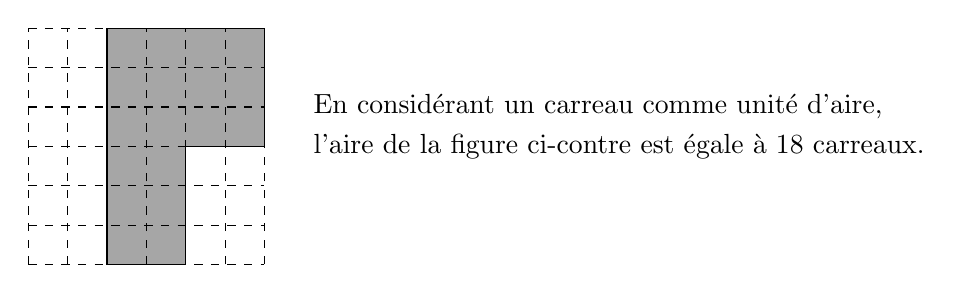
\begin{tikzpicture}[scale=0.5]
        \draw[fill=black!35!white] (2,0) -- (4,0) -- (4,3) -- (6,3) -- (6,6) -- (2,6) -- cycle;
        \draw[dashed] (0,0) grid (6,6);
        \node[right] at (7,4) {En considérant un carreau comme unité d'aire,};
        \node[right] at (7,3) {l'aire de la figure ci-contre est égale à 18 carreaux.};
    \end{tikzpicture}
    \end{center}%
}

\partie{Formules de mesures d'aires}

\begin{tabular}{|c|c|c|c|}\hline
    Forme géométrique & Formule & Formule abrégée & Schéma  \\\hline
    Carré & côté $\times$ côté & $c \times c$ & 
    \makecell{\begin{tikzpicture}
        \draw (0,0) -- (0,1) -- (1,1) -- (1,0) -- cycle;
        \node[above] at (0.5,1) {$c$};
        \draw (0.5,0.9) -- (0.5,1.1);
        \draw (0.5,0.1) -- (0.5,-0.1);
        \draw (0.1,0.5) -- (-0.1,0.5);
        \draw (1.1,0.5) -- (0.9,0.5);
    \end{tikzpicture}} \\\hline
    Rectangle & Longueur $\times$ largeur & $L \times \ell$ & 
    \makecell{\begin{tikzpicture}
        \draw (0,0) -- (2,0) -- (2,1) -- (0,1) -- cycle;
        \node[above] at (1,1) {\small{$L$}};
        \node[right] at (2,0.5) {$\ell$};
        \draw (1,0.9) -- (1,1.1) (1,0.1) -- (1,-0.1);
        \draw (-0.1,0.45) -- (0.1,0.45) (-0.1,0.55) -- (0.1,0.55);
        \draw (1.9,0.45) -- (2.1,0.45) (1.9,0.55) -- (2.1,0.55);
    \end{tikzpicture}} \\\hline
    Losange & (grande diagonale $\times$ petite diagonale) $\div 2$ & $(D \times d)\div2$ & 
    \makecell{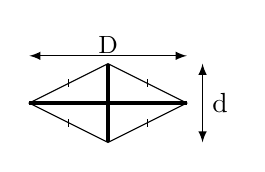
\begin{tikzpicture}
        \draw (-1,0) -- (0,0.5) -- (1,0) -- (0,-0.5) -- cycle;
        \node[above] at (0,0.5) {\small{D}};
        \node[right] at (1.2,0) {d};
        \draw (-0.5, -0.3) -- (-0.5,-0.2);
        \draw (-0.5, 0.3) -- (-0.5,0.2);
        \draw (0.5, -0.3) -- (0.5,-0.2);
        \draw (0.5, 0.3) -- (0.5,0.2);
        \draw[very thick] (-1,0) -- (1,0) (0,0.5) -- (0,-0.5);
        \draw[latex-latex] (1.2,0.5) -- (1.2,-0.5);
        \draw[latex-latex] (-1,0.6) -- (1,0.6);
    \end{tikzpicture}} \\\hline
    Triangle & (base $\times$ hauteur) $\div 2$ & $(b\times h)\div 2$ & 
    \makecell{\begin{tikzpicture}
        \node[above] at (0,0.8) {\phantom{e}};
        \coordinate (A) at (0,0);
        \coordinate (B) at (1,0);
        \coordinate (C) at (0.2,1);
        \coordinate (H) at ($(A)!(C)!(B)$);
        \draw (A) -- (B) -- (C) -- cycle;
        \draw[thick] (C) -- (H);
        \node[right] at ($(C)!0.5!(H)$) {\small{$h$}};
        \node[below] at ($(A)!0.5!(B)$) {\small{$b$}};
    \end{tikzpicture}} \\\hline
    Disque & $\pi \times $ rayon $\times$ rayon & $\pi \times r \times r$ & 
    \makecell{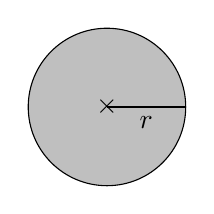
\begin{tikzpicture}
        \draw[fill=lightgray] (0,0) circle (1);
        \node at (0,0) {$\times$};
        \draw (0,0) -- (1,0);
        \node[below] at (0.5,0) {$r$};
    \end{tikzpicture}}\\\hline
\end{tabular}

\remarque{Lors de l'utilisation d'une formule, toutes les valeurs doivent avoir la même unité.}
\remarque{La valeur $\pi$ peut être approximée par le nombre \num{3,14}. }

\clearpage
\partie{Conversion d'unités d'aires}

\definition{Un mètre carré est l'aire d'un carré d'un mètre de côté.}

\convention{L'unité légale de l'aire d'une surface est le mètre carré (noté \unit{m\squared}).}\\

\par Pour convertir les unités d'aires entre elles, on utilise le tableau ci-dessous, en utilisant les règles suivantes :
\begin{itemize}
    \item Le chiffre des unités est placée dans la colonne de droite de l'unité d'origine.
    \item On complète par des 0 jusqu'à arriver à la colonne de droite de la nouvelle unité, et on place la virgule à cet endroit lorsqu'elle est nécessaire.
\end{itemize}

\begin{center}
\begin{tabular}{|*{14}{p{0.8cm}|}}\hline
    \multicolumn{2}{|c|}{\phantom{$a^{2^2}$}\unit{km\squared}\phantom{$a^{2^2}$}} & \multicolumn{2}{|c|}{\unit{hm\squared}} & \multicolumn{2}{|c|}{\unit{dam\squared}} & \multicolumn{2}{|c|}{\unit{m\squared}} & \multicolumn{2}{|c|}{\unit{dm\squared}} & \multicolumn{2}{|c|}{\unit{cm\squared}} & \multicolumn{2}{|c|}{\unit{mm\squared}} \\\hline
     & & & & & & & & & & & & & \makecell{\vspace{2cm}} \\\hline 
\end{tabular}
\end{center}

\begin{listedexemples}
    \item \qty{13}{hm\squared} = .......... \unit{m\squared}
    \item \qty{2,5}{km\squared} = .......... \unit{dm\squared}
    \item \qty{0,02}{dm\squared} = .......... \unit{dam\squared}
\end{listedexemples}

\remarque{Un hectare (noté \unit{ha}) est égal à \qty{1}{hm\squared}.\\ Un are (noté \unit{a}) est égal à \qty{1}{dam\squared}.}

\clearpage
\begin{questions}
    \exercice\\ Calculer l'aire des figures suivantes
        \question Un carré de côté \qty{3}{cm}
        \question Un rectangle de largeur \qty{7}{dm} et de longueur \qty{9}{cm}
        \question Un disque de rayon \qty{3}{cm}
        \question Un disque de diamètre \qty{4}{m}
        \question Un losange de petite diagonale \qty{3}{km} et de grande diagonale \qty{40}{hm}
        \question Un triangle de base \qty{4}{cm} et de hauteur \qty{8}{cm}
    \exercice\\ Convertir
        \question \qty{3,2}{km\squared} en \unit{dm\squared}
        \question \qty{80}{dm\squared} en \unit{dam\squared}
        \question \qty{3,9876}{ha} en \unit {cm\squared}
        \question \qty{5,2764}{dam\squared} en \unit{mm\squared}
        \question \qty{7,2846}{m\squared} en \unit {cm\squared}
        \question \qty{1,0023}{km\squared} en \unit{m\squared}
    \exercice\\ Calculer l'aire des figures suivantes
        \begin{center}
            \begin{tabular}{p{7cm}|p{7cm}}
                \geocell{
                    \rectangleCODAGE{0,0}{3}{1}{||}{|}
                    \node[below] at (0,1.5) {}
                } &  \\\hline
                \geocell{}
            \end{tabular}
        \end{center}
\end{questions}

\end{document}
